\section{Markov chains}

Discrete-time stochastic process $\{ X_n = X(t_n) \}^{\infty}_{n=0}$ is called \textbf{Markov Process}, if ${\rm Pr} \{ X_n = i_n | X_{n-1} = i_{n-1} \}$, here $i_k$ belongs to the state space of the random variable $X$. Of this state space of $X$ is \textbf{finite} then it's a \textbf{finite Markov Chain}. \textbf{One-step transition probability} $p_{ji}(n) = {\rm Pr \{X_{n+1} = j | X_n = i \}}$. If $p_{ji}(n) \equiv p_{ji} = {\rm const}$, the Markov chain is \textbf{stationary}. Note that $\sum_j p_{ji} = 1$.  

We can define a transition matrix
\begin{center}
    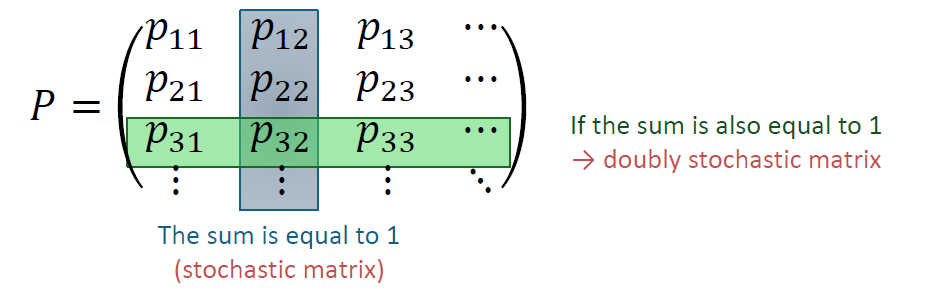
\includegraphics[width=250pt]{images/transition matrix.png}
\end{center}

If $P$ is stochastic matrix, then $P^{n}$ is a stochastic matrix as well. If $P$ is doubly stochastic matrix, then $P^n$ is a doubly stochastic matrix as well.

We can also define $n$-step transition probability i.e. the probability of transferring from state $i$ to state $j$ in $n$ time steps
\begin{equation*}
    p_{ji}^{(n)} = {\rm Pr} \{ X_n = j | X_0 = i \}
\end{equation*}
Then clearly
\begin{align*}
    &n = 0 \quad \Rightarrow \quad p_{ji}^{(0)}=\delta_{ji} \\
    &n = 1 \quad \Rightarrow \quad p_{ji}^{(1)}=p_{ji}
\end{align*}

\subsection{Chapman-Kolmogorov equation}
The Chapman-Kolmogorov equation relates the $n$-step transition porobability with the $s$-step and $(n-s)$-step transition probabilities:

\begin{align}
p^{(n)}_{ji}
&= \Pr\{ X_n = j \mid X_0 = i \} \\[0.5em]
&= \sum_{k=1}^{\infty} 
   \Pr\{ X_n = j,\; X_s = k \mid X_0 = i \} \\[0.5em]
&= \sum_{k=1}^{\infty} 
   \Pr\{ X_n = j \mid X_s = k,\; X_0 = i \}
   \Pr\{ X_s = k \mid X_0 = i \} \\[0.5em]
&= \sum_{k=1}^{\infty} 
   \Pr\{ X_n = j \mid X_s = k \}
   \Pr\{ X_s = k \mid X_0 = i \} \\[0.5em]
&= \sum_{k=1}^{\infty} 
   p^{(n-s)}_{jk}\, p^{(s)}_{ki}.
\end{align}

Thus
\begin{equation*}
    p_{ji}^{(n)} = \sum_{k=1}^{\infty} p_{jk}^{(n-s)} p_{ki}^{(s)}
\end{equation*}
or in a matrix form: $P^{(n)} = P^{(n-s)} \cdot P^{s}$, the notice that $P^{(n)} = P^{n}$


\subsection{Classification of states}
\textbf{Irreducable Markov chain} is such that from any state it is possible to reach any other state is some number of steps. Otherwise it is \textbf{reducable} i.e. there either exist some disjoint parts or there is a a way one relation between some states.

\begin{center}
    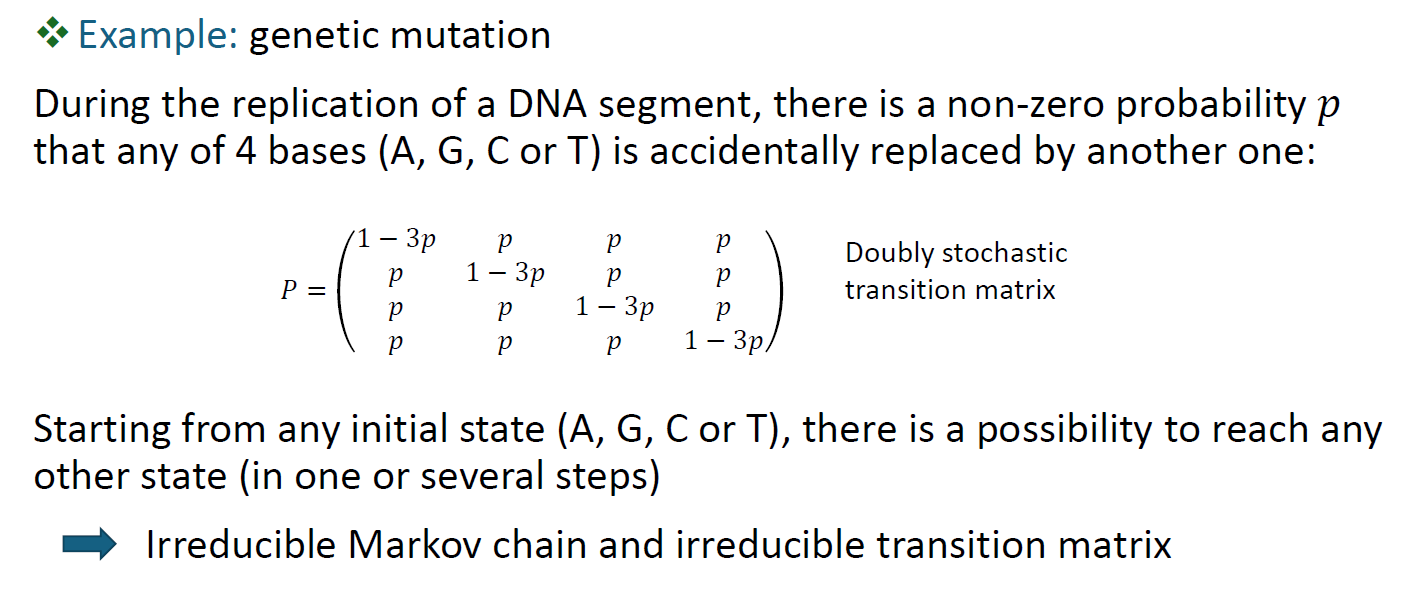
\includegraphics[width=300pt]{images/example genetic mutation.png}
\end{center}

\textbf{Communicating states} are those who can reach one another in both directions, hence the notation $i \xrightarrow j$. Likewise, \textbf{communication classes} are just sets of all the states that can communicate. If there exists multiple more than one communication class then the state is reducable.

\begin{center}
    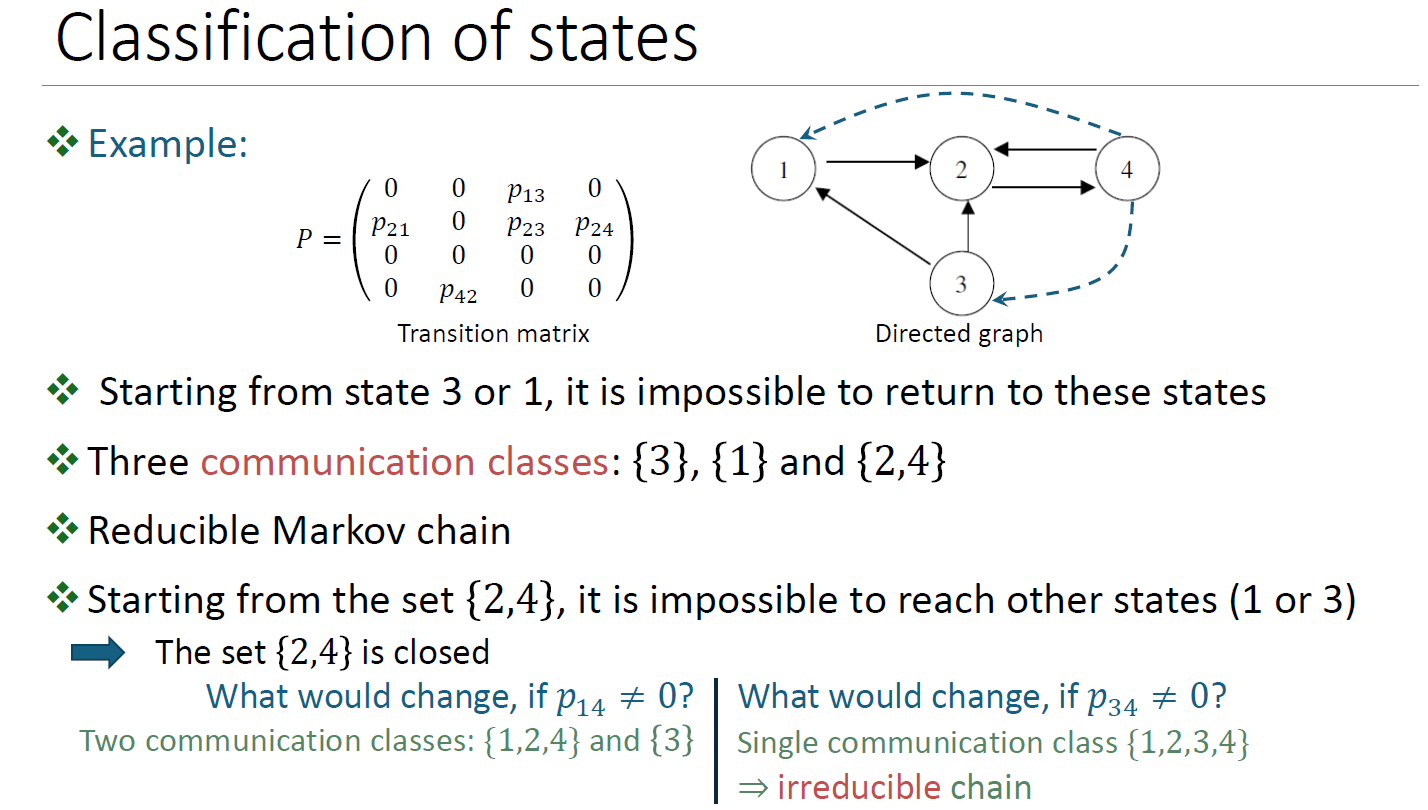
\includegraphics[width=300pt]{images/Example communication class.png}
\end{center}

\textbf{Absorbing boundaries} are such boundaries which when enterred are never left i.e. $p_{ii} = 1$. If there exists absorbing boundaries, then there are several communication classes and thus the markov chain is reducable.

\textbf{Period of a state} $d_i$ of state $i$ is the greatest common divisor of all integers $n \geq 1$, for which $p^{n}_{ii} > 0$
\begin{itemize}
    \item If $d_i > 1$, state $i$ is \textbf{periodic} with period $d_i$
    \item If $d_i = 1$, state $i$ is \textbf{aperiodic}
    \item If $p_{ii}^{n} = 0$ for all $n$, the period is defined as $d_i = 0$
\end{itemize} 

\begin{center}
    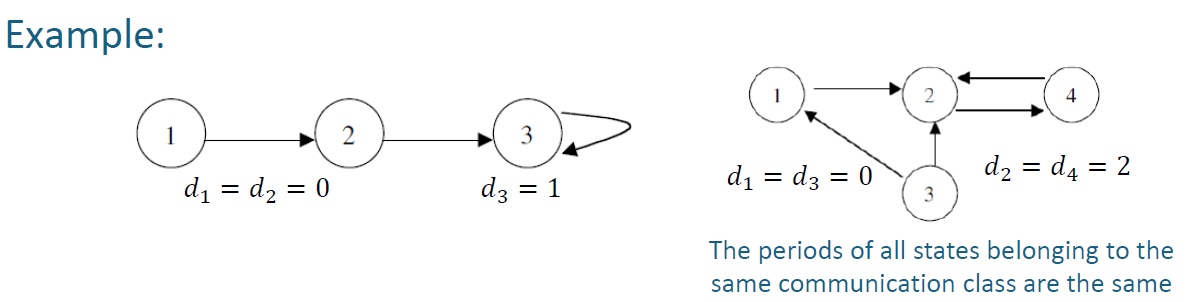
\includegraphics[width=300pt]{images/example period of states.png}
\end{center}

\begin{center}
    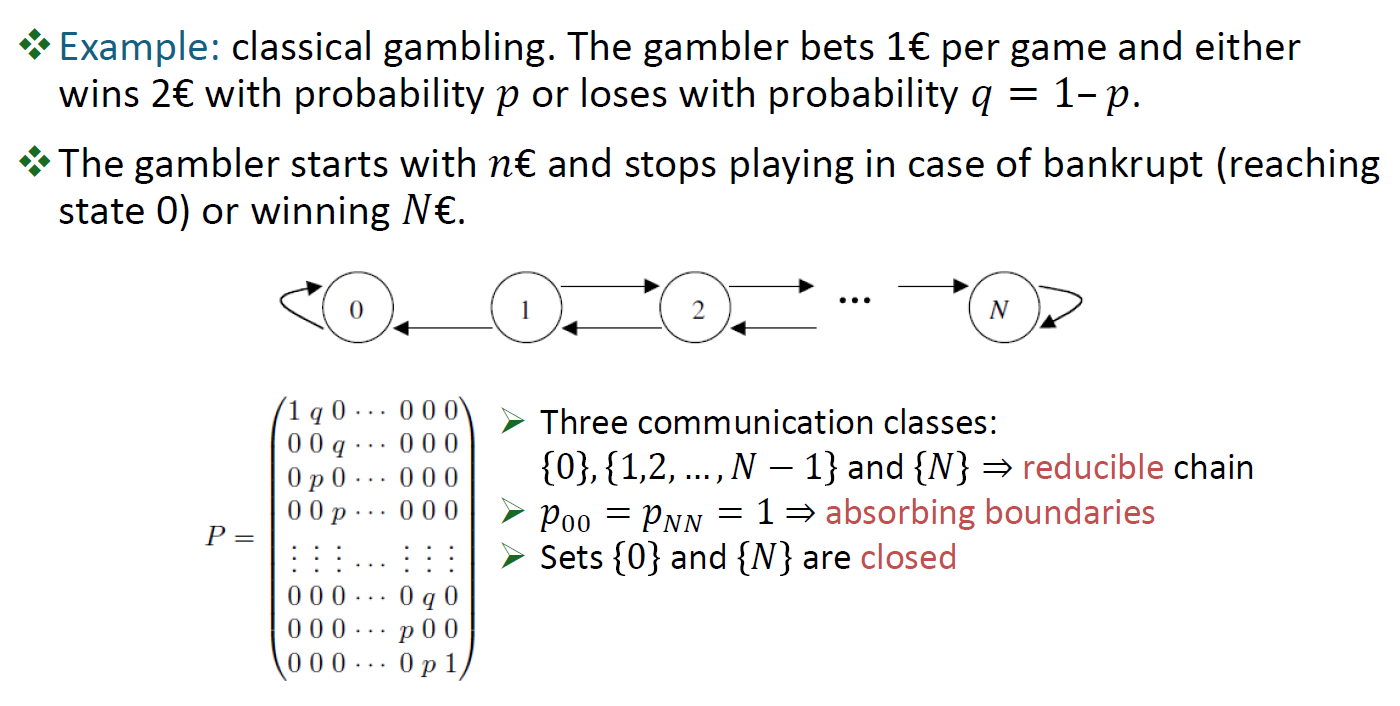
\includegraphics[width=300pt]{images/example gambling.png}
\end{center}

\begin{center}
    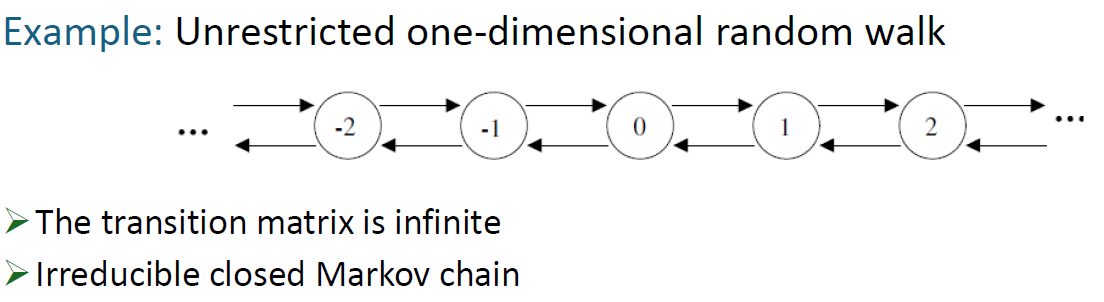
\includegraphics[width=300pt]{images/example random walk.png}
\end{center}

\begin{center}
    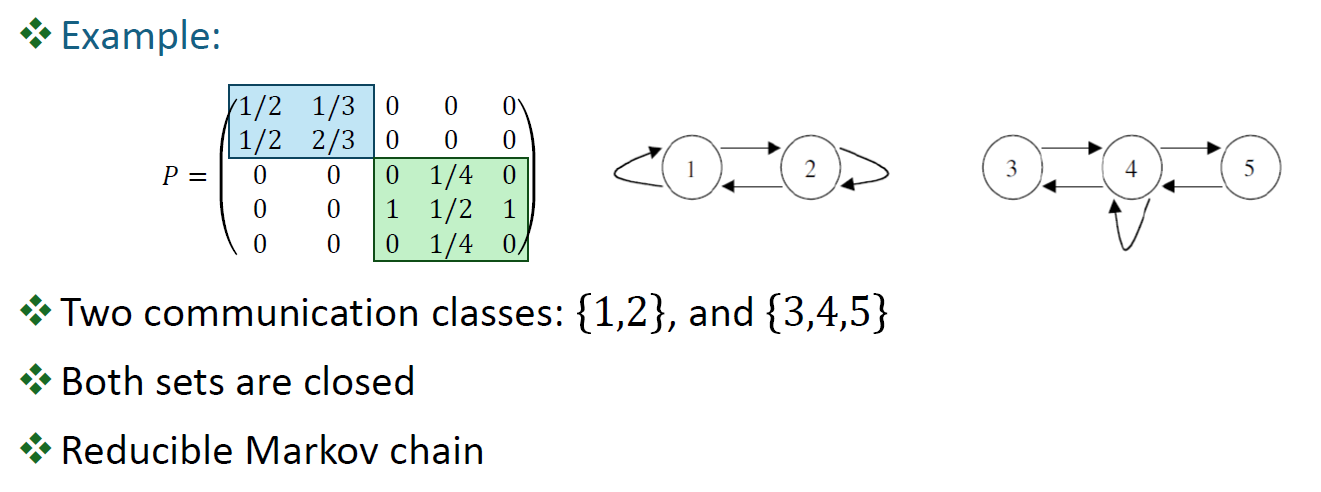
\includegraphics[width=300pt]{images/example classification of states.png}
\end{center}

\begin{center}
    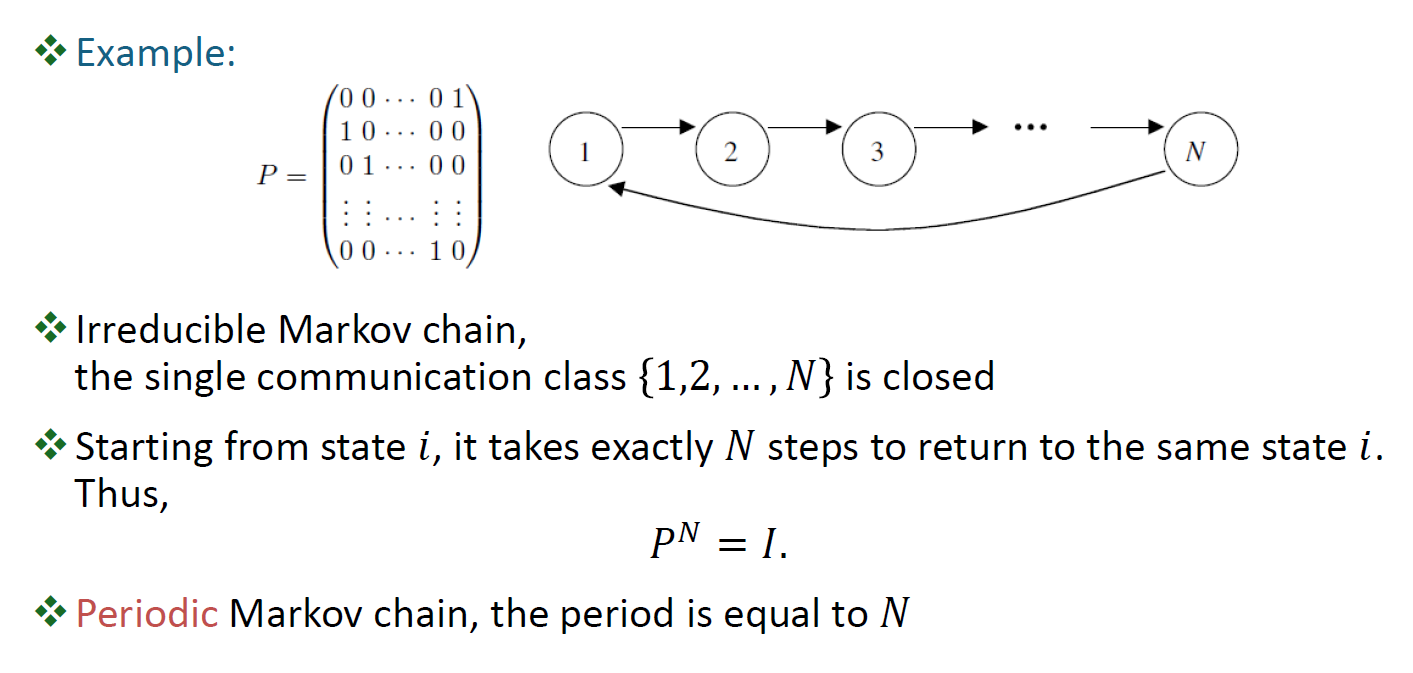
\includegraphics[width=300pt]{images/example periodic markov chain.png}
\end{center}


\subsection{First-return time}
Let $f^{n}_{ii}$ denote the probability that random variable $X$ aquired again its initial value $X_0 = i$ after $n$ steps:

\begin{equation*}
    f_{ii}^{(n)} = {\rm Pr} \{ X_n = i, X_m \neq i, m = 1,2, \dots, n-1 | X_0=1 \}
\end{equation*}
Note that $f_{ii}^{1} = p_{ii}$

We can now define the following. \textbf{recurent} state is such a state that will be inifnitely visited, but a \textbf{transient} state is such which might be visited finite number of times, but eventually it will not be visited ever again.

\begin{itemize}
    \item If $\sum_{n=1}^{\infty} f_{ii}^{n} = 1$, state $i$ is \textbf{recurent}
    \item If $\sum_{n=1}^{\infty} f_{ii}^{n} < 1$, state $i$ is \textbf{transient}
\end{itemize}

For a recurent state we can define a new random variable $T_{ii}$, whose elements $T_{ii}^{n} = n \in \mathbb{N}$ are acquired with probabilities $f_{ii}^{(n)}$ and is called a \textbf{first return time}. In addition, for the recurrent state, we can define the \textbf{mean recurrence} (or \textbf{first-return}) time:
\begin{equation*}
    E(T_{ii}) \equiv \langle T_{ii} \rangle = \sum_{n=1}^{\infty} n f_{ii}^{(n)}
\end{equation*}

\begin{center}
    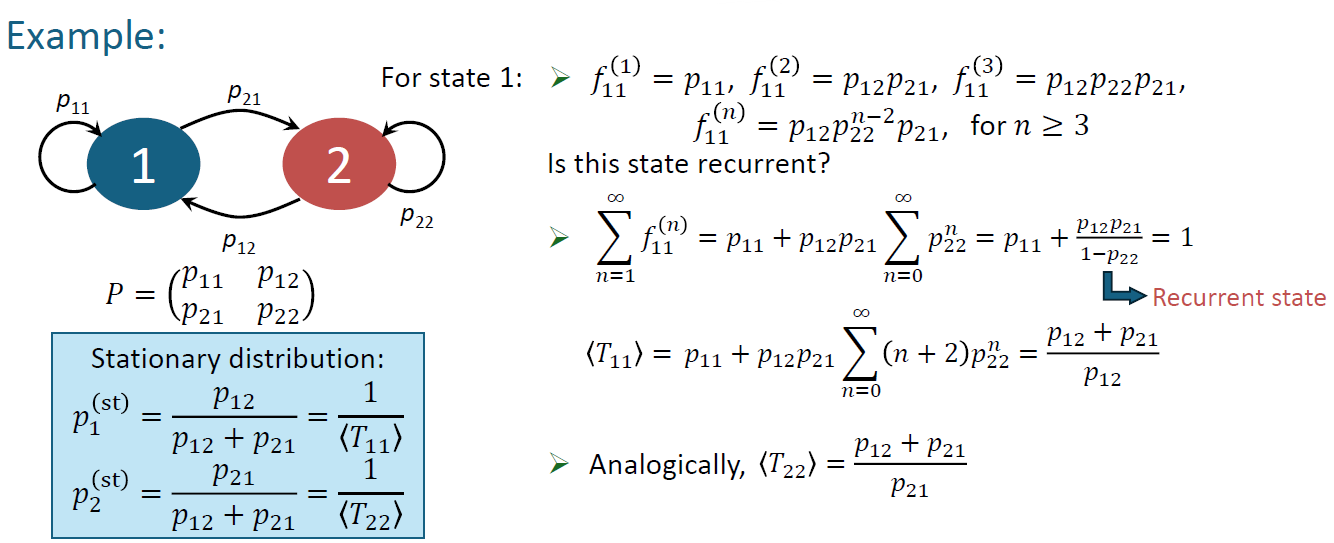
\includegraphics[width=300pt]{images/example mean passage time.png}
\end{center}

\subsection*{Basic Limit theorem}
If ${X_n}$ is a recurrent, irreducable, and aperiodic Markov chain with one-step transition probabilities $p_{ij}$, then 
\begin{equation*}
    \frac{1}{\langle T_{ii} \rangle} = \lim_{n \rightarrow \infty} p_{ij}^{(n)} = p_i^{\rm (st)}
\end{equation*}

If ${X_n}$ is a recurrent, irreducable, and periodic Markov chain with period $d>1$, then

\begin{equation*}
    \lim_{n \rightarrow \infty} p_{ii}^{nd} = \frac{d}{ \langle T_{ii} \rangle} 
\end{equation*}
and $p^{(m)}_{ii} = 0$ if $m$ is not a multiple of $d$.

\begin{center}
    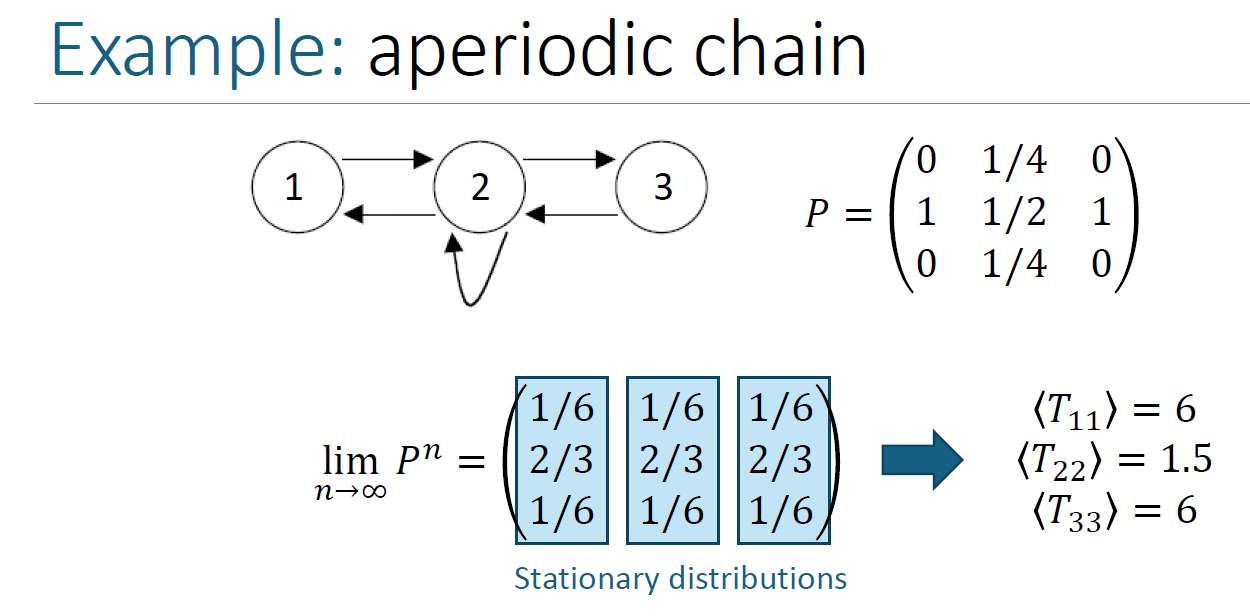
\includegraphics[width=300pt]{images/example aperioc chain.png}
\end{center}

\begin{center}
    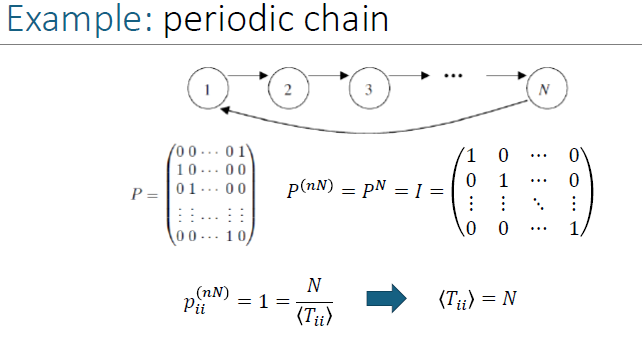
\includegraphics[width=300pt]{images/example periodic chain.png}
\end{center}


\section{Mean first-passage time}
Define \textbf{fist-passage proobability} $f_{ji}^{(n)}$ that starting from state $X_0=i$ after $n$ steps you end up at state $j$

\begin{equation*}
    f_{ji}^{(n)} = {\rm Pr} \{ X_n = j, X_m \neq j, m= 1,2, \dots, n-1 | X_0 = i\}
\end{equation*}

Note that
\begin{equation*}
    0 \leq \sum_{n = 1}^{\infty} f_{ji}^{(n)} \leq 1
\end{equation*}

Then, the mean time of first passage from state $i$ to state $j$ is
\begin{equation*}
    \langle T_{ji} \rangle = \sum_{n=1}^{\infty} n f_{ji}^{(n)}
\end{equation*}

This is more easily calculable. Define
\begin{equation*}
    T = 
    \begin{bmatrix}
        \langle T_{11} \rangle & \langle T_{12} \rangle & \dots & \langle T_{1N} \rangle \\
        \langle T_{21} \rangle & \langle T_{22} \rangle & \dots & \langle T_{2N} \rangle \\
        \vdots                 & \vdots                 & \vdots & \vdots \\
        \langle T_{N1} \rangle & \langle T_{N2} \rangle & \dots & \langle T_{NN} \rangle
    \end{bmatrix}
\end{equation*}

The in matrix form we have the following identity
\begin{equation*}
    T = E + (T - {\rm diag}(T)) \cdot P
\end{equation*}

where $T$ is the matrix of mean times, $E$ is matrix of ones (not identity, just every element is 1) and $P$ is a transition matrix.

\begin{center}
    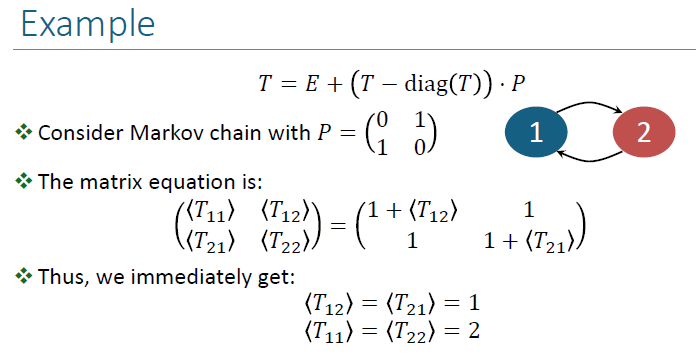
\includegraphics[width=300pt]{images/example mean time matrix.png}
\end{center}